\documentclass[12pt]{article}

\title{Química Inorgánica}
\author{Abel Doñate}
\date{}

\usepackage{amsmath}
\usepackage{chemfig}
\usepackage{graphicx}
\usepackage{subcaption}
\graphicspath{ {./images/} }
\usepackage{wrapfig}
\usepackage{enumitem}
\usepackage{mathtools}
\usepackage{hyperref}



%Geometry
\usepackage{geometry}
\geometry{a4paper, margin=1in}


\begin{document}

\maketitle
\tableofcontents
\newpage

\section{Cuántica}
	\subsection{Problemas a los que se enfrentaban}
	\begin{itemize}
		\item Teorema de equipartición de la $E$ incorrecta para moléculas poliatómicas
		\item Existencia de espectros atómicos (H) $\bar{\nu}=R(\frac{1}{2^2}-\frac{1}{2^n})$ (Serie de Balmer)
		\item Radiación del cuerpo negro (Planck) 
	\end{itemize}
	Surgen teorías como el Efecto Fotoeléctrico $h\nu=h\nu_0+E_c$, la Hipótesis de De Broglie $\lambda=h/p$ y el Modelo de Rutherford.
		
	\subsection{Modelo de Bohr}
	\begin{enumerate}[label=\arabic*)]
		\item $e^-$ ocupa órbitas estacionarias (no emiten $E$)
		\item $L=mvr=\lambda \hbar$ cuantizado 
		\item Pueden cambiar de órbita (explica serie de Balmer)
	\end{enumerate}
	
	\subsection{Postulados de la Mecánica Cuántica}
	\begin{itemize}
		\item[1)] $\Psi(q_1, \cdots,q_n,t)$ función de onda
		\item[2)] $\hat{H}\Psi = -\frac{\hbar}{i}\frac{\partial\Psi}{\partial t}$  (Schrödinger)
		\item[3)] Normalización $\implies$   $\int_{-\infty}^\infty{\Psi \Psi^\ast d\tau1=1}$
		\item[4)] Toda propiedad observable tiene asociado un operador, que aplicado a la función da como resultado un número real.
		\item[5)] $<p>= \int_{-\infty}^\infty{\Psi \hat{p} \Psi^\ast d\tau}$   ($\Psi$ norlmalizado)
	\end{itemize}
	
	\subsection{Partícula en un pozo de potencial. Efecto túnel}
		\begin{figure}[h!]
\centering
\begin{subfigure}[b]{0.45\linewidth}
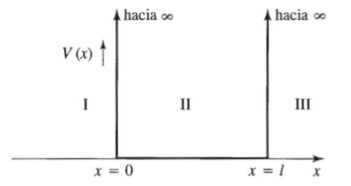
\includegraphics[width=\linewidth]{Pozo_potencial_infinito}
\caption{Pozo de potencial infinito}
\label{fig:westminster_lateral}
\end{subfigure}
\begin{subfigure}[b]{0.45\linewidth}
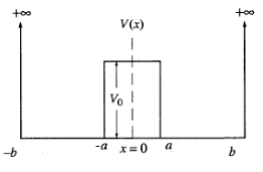
\includegraphics[width=\linewidth]{Pozo_potencial_finito}
\caption{Pozo de potencial finito}
\label{fig:westminster_aerea}
\end{subfigure}
\label{fig:westminster}
\end{figure}
El potencial es $\infty$ en $I$ y $III$ y $0$ en $II$. La solución es una onda sinusoidal en $II$ (normalizar e igualar en $0$ y $l$) \\

Cuando el potencial es finito se da el efecto túnel, ya que existe una pequeña probabilidad de que la partícula se encuentre fuera del pozo.		

\newpage	
\section{Sistema Periódico}
\subsection{Configuración electrónica}
Escribimos la configuración electrónica como $1s^22s^2\cdots nc^\alpha$.\\
Siempre ordenamos por niveles (pero teniendo en cuenta el diagrama de Moeller)\\ \\
Hay 2 excepciones donde se produce la promoción electrónica:
\begin{itemize}
	\item Cr: $[Ar]\ 3d^54s^1$
	\item Cu: $[Ar]\ 3d^{10}4s^1$
\end{itemize}

\subsection{Números cuánticos}
\begin{itemize}
	\item $n$ natural (capa o nivel)          N. c. principal
	\item $l = 0,\cdots n-1$ (grupo)          N. c. azimutal
	\item $m = -l, \cdots l$ (tipo de orbital) N. c. magnético
	\item $s/m_s=1/2, -1/2$                   N. c. de spin
\end{itemize}

\subsubsection{Reglas de Slater}
La carga nuclear efectiva viene dada por $z^*=z-\sum\sigma$ \\

Poner configuración en forma $(1s^2)(2s^2)...(ns\ np)(nd\ nf)$
\begin{itemize}
	\item Si es $s,p$
	\begin{itemize}
		\item[-] $\sigma= 0.35$ en esa capa ($\sigma= 0.31$ si es $1s$)
		\item[-] $\sigma= 0.85$ en la capa inferior 
		\item[-] $\sigma=1$ en los orbitales a la izquierda
	\end{itemize}
	\item Si es $d,f$
	\begin{itemize}
		\item[-] $\sigma= 0.35$ en ese orbital
		\item[-] $\sigma=1$ en los orbitales a la izquierda
	\end{itemize}
\end{itemize}

La energía de un átomo es \(E= E_0\sum\displaystyle\left(\frac{z^*}{n_i}\right)^2\)
\subsection{Propiedades Periódicas}
\begin{itemize}
	\item EI (Energía de Ionización). E para formar el catión $\uparrow \rightarrow $
	\item AE (Afinidad Electrónica). E desprendida al formar un anión $\uparrow \rightarrow$
	\item Radio Atómico (depende de la definición y del compuesto). $\downarrow \leftarrow$
	\item Caracter metálico $\downarrow \leftarrow$
	\item Electronegatividad $\uparrow \rightarrow$
\end{itemize}

\subsubsection{Efecto del par inerte}
Explica la tendencia de un par de $e^-$ de un orbital $s$ de un nivel externo a no ser utilizado para formar un un compuesto.
\[Al\ \rightarrow \ Al^{+3}+3e^-\ \ \ \ (3s^23p^1)\]
\[In\ \rightarrow \ In^{+}+e^-\ \ \ \ (5s^25p^1)\]

\subsubsection{Relaciones diagonales}
\begin{itemize}
	\item[-] $Li\leftrightarrow Mg$ forman nitruro, nitratos y carbonatos inestables a $T^a$ alta. Misma facilidad para formar sales hidratadas.
	\item[-] $Be\leftrightarrow Al$ forman óxidos anfóteros (ácidos/bases). $BCl_2, AlCl_3$ catalizadores en Fiedel Crafts.
	\item[-] $B\leftrightarrow Si$ forman óxidos de carácter ácido y comportamiento vítreo. Boratos y silicatos parecidos.
\end{itemize}

\section{Enlace covalente}
\subsection{Estructuras de Lewis}
Hasta el segundo periodo se debe seguir la regla del octeto.\\
Moléculas como el Ozono ($O_3$) tifenen varias formas canónicas 
%\chemfig
\subsection{Hibridación (Modelo TEV)}
El número de orbitales híbridos se calcula como $No \ hibridos=No \ enlaces + No \ pares \ libres$.\\
\begin{table}[h!]
\begin{tabular}{lll}
\underline{Híbridos} & \underline{Tipo de hibridación} & \underline{Geometría}                                     \\
2                 & $sp/sd\ (\sigma)$                   & lineal                                              \\
3                 & $sp^2\ (\sigma, \pi)$                    & trigonal plana/angular                              \\
4                 & $sp^3/sd^3\ (\sigma, 2\pi)$               & tetraédrica/piramidal trigonal/angular              \\
5                 & $sp^3d/dsp^3$             & bipirámide trigonal/silla (balancín)/forma T/lineal \\
6                 & $sp^3d^2/d^2sp^3$         & octaédrica/pirámide cuadrangular/planicuadrada     
\end{tabular}
\end{table}
\subsection{Modelo RPECV}
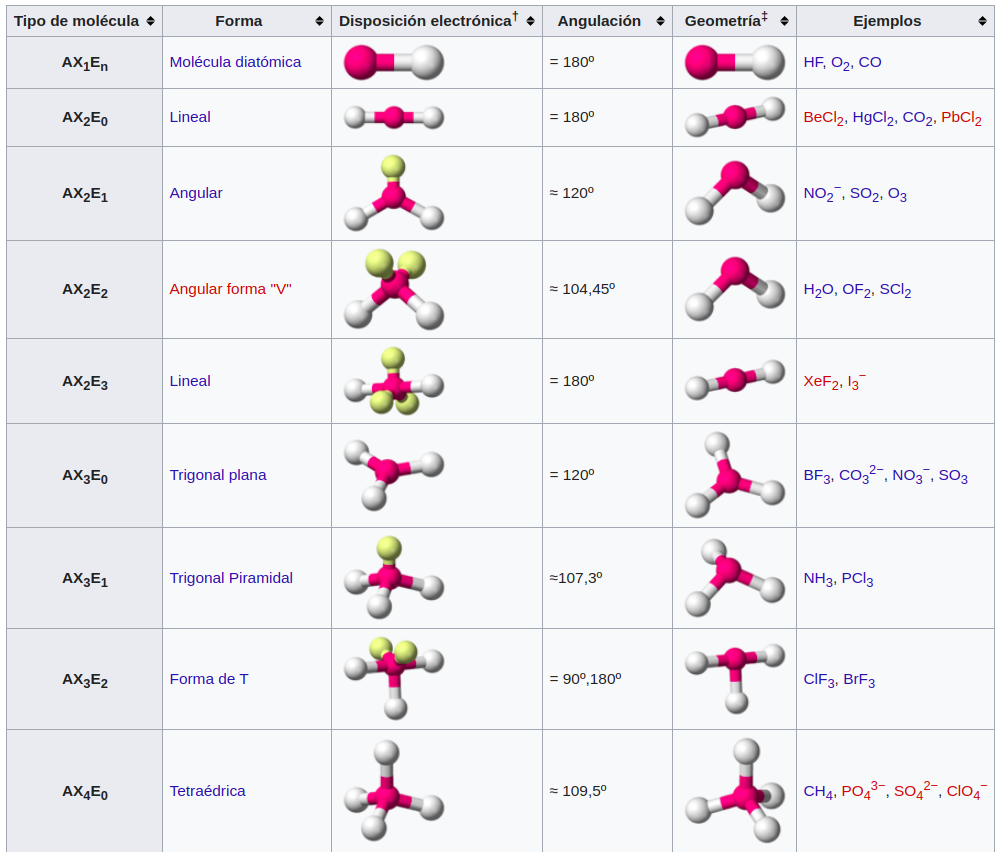
\includegraphics[scale=0.45]{Geometria1.png}\\
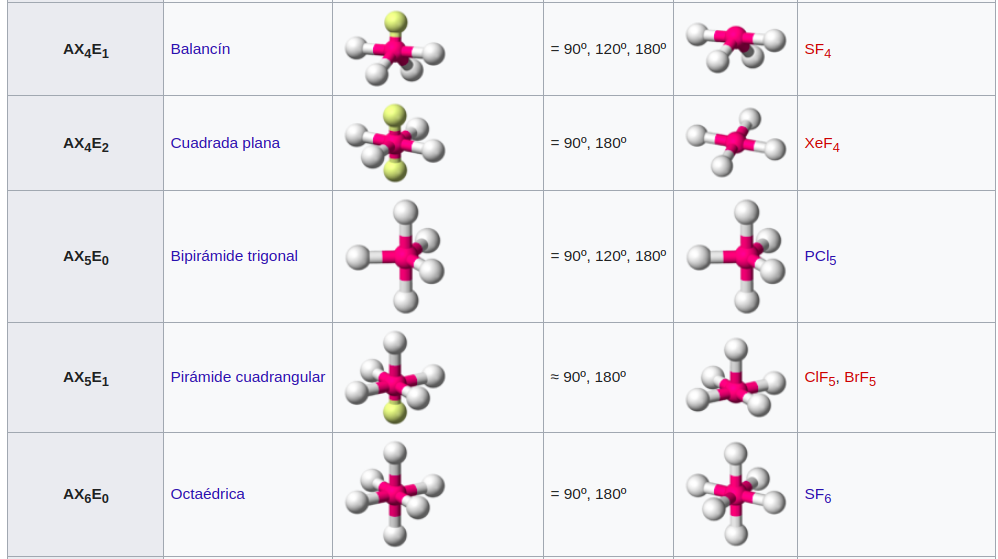
\includegraphics[scale=0.45]{Geometria2.png}\\
\subsection{Teoría de orbitales moleculares. Combinación lineal de los orbitales atómicos (CLOA)}
Se supone que $\psi_j=\sum{c_{ij}\phi_i}$ es una combinación lineal de los orbitales simples $\phi_i$.\\
Los orbitales siguen las siguientes reglas:
\begin{itemize}
	\item[-] $OM$ (Orbitales Moleculares) $= OA$ (Orbitales Atómicos)
	\item[-] $OM$ enlazantes y $OM$ antienlazantes (*)
	\item[-] Principio de Aufbau
	\item[-] Principio de exclusión de Pauli
	\item[-] Regla de Hund
	\item[-] Especies más estables tienen más orbitales enlazantes
	\item[-] Hasta el N se llenan primero los $\pi_x, \pi_y$, después del O $\sigma_z$
\end{itemize}
El orden del enlace ($OE$) será:
\[OE \ \text{(Orden del Enlace)} = \frac{OM - OM^*}{2}\]
Cuanto mayor sea el $OE$, más estable será la molécula \\
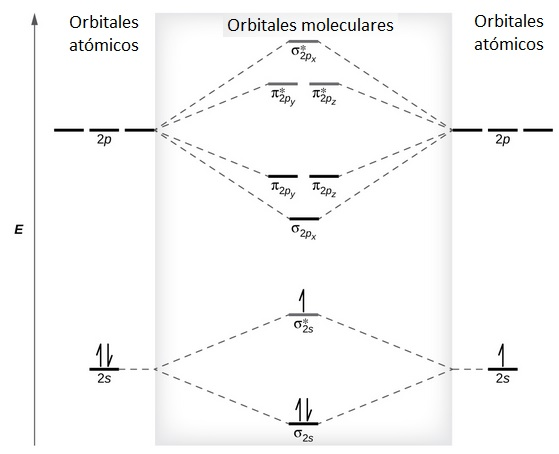
\includegraphics[scale=0.4]{Orbitales_moleculares}
\subsection{Propiedades de los enlaces}
\subsubsection{Electronegatividad}
Existe la escala de Pauling, calculada de la siguiente manera:
\[X_A-X_B=0.208\sqrt{\Delta_{A-B}}\ \ \ \ \ donde \ \ \Delta_{A-B}=D_{A-B}-\frac{1}{2}(D_{A-A}+D_{B-B})\]
Se le asigna a $X_F$ (el de mayor electronegatividad) el valor arbitrario de 4.
\subsubsection{Carácter iónico}
Se asigna un porcentaje de carácter iónico a cada elemento (fórmula en la hoja).\\
También se puede calcular con la siguiente fórmula:
\[\% ionico=\frac{\mu_{exp}}{\mu_{teo}}*100 \]
\subsubsection{Momento dipolar. Polaridad}
A cada enlace se re asocia un momento dipolar $\vec{\mu_i}$ que apunta hacia el átomo más electronegativo.\\
Al sumar los momentos dipolares 
\( \left\{
\begin{array}{ccc}
	\sum{\vec{\mu_i}}=\vec{0}  &  \implies  &  apolar\\
	\sum{\vec{\mu_i}}\neq\vec{0}  &  \implies  &  polar
\end{array} 
\right.
\)\\
\\
Podemos calcular  el momento dipolar \(\mu=dq\), donde d es la distancia entre los átomos.
\subsubsection{Energía y distancia del enlace}
\begin{wrapfigure}{l}{0.4\textwidth}
    \centering
    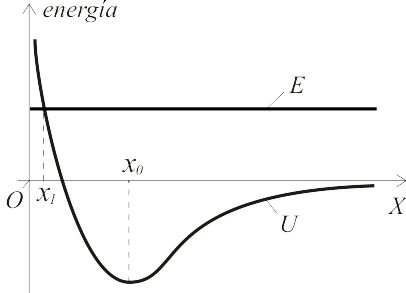
\includegraphics[width=0.35\textwidth]{Distancia_enlace}
\end{wrapfigure}
Distancia de mínima energía favorecerá la formación del enlace.\\
\\
Existen tablas ponderadas de distancia y de energía de los enlaces.
\\ \\ \\ \\ \\ \\ 

\subsection{Enlaces intermoleculares. Fuerzas de Van der Wals}
\begin{itemize}
	\item Dipolo permanente - Dipolo permanente. \\
	Se forman entre moléculas polares. Son las más fuertes si M es pequeña.\\
	Un caso particular son los puentes de Hidrógeno, que se forman cuando existe un enlace intermolecular entre H y N, O, F.
	\item Dipolo permanente - Dipolo inducido.
	Se forman entre moléculas polares y apolares.
	\item Dipolo instantáneo - Dipolo instantáneo o Fuerzas de dispersión de London.\\
	Se forman entre moléculas apolares. Aumenta la fuerza con M.
	
\end{itemize}

Las consecuencias de estas fuerzas son las siguientes:
\begin{itemize}
	\item[-] Variación regular en las propiedades físicas ($T_f, T_e$).
	\item[-] Solubilidad en disolventes de su misma polaridad.
	\item[-] Formación de micelas o bicapas.
\end{itemize}

\section{Enlace metálico}
	\subsection{Direcciones y Planos}
La notación para direcciones es $[\alpha \ \beta \ \gamma]$, donde las 			cordenadas $[1\ 0\ 0] = \vec{a}...$, etc y $\alpha, \beta,\gamma$ son enteros.\\ \\
Para los planos se utiliza la notación de Miller $(\alpha \ \beta \ \gamma)$, donde estos son los inversos de los cortes del plano con los respectivos ejes de coordenadas.

	\subsection{Polimorfismo y alotropía}
El \textbf{Polimorfismo} se dacuando una sustancia presenta diferentes estructuras cristalinas en función de $T, P$. Cada estructura es una \textbf{Forma Alotrópica}

	\subsection{Motivo y Red de Bravais}
El \textbf{motivo} es el conjunto de átomos de un cristal que se asocia a cada nodo. \[Motivo=\frac{atomos}{P.\ reticulares} \ (atomos\ de \ X)\]

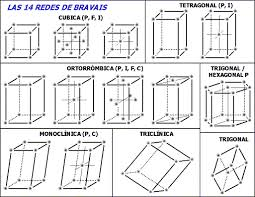
\includegraphics[scale=0.7]{Bravais}

	\subsection{Principales Empaquetamientos}
Los principares empaquetamientos son los siguientes:
\begin{table}[h!]
\begin{tabular}{lll}
\underline{Tipo} & \underline{Características} & \underline{Imagen}                                     \\
BCC & $FE=0.68$ , $IC=8$ y $\sqrt{3}a=4R$& 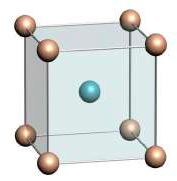
\includegraphics[width=0.1\textwidth]{BCC}                             \\
FCC & $FE=0.74$ , $IC=12$ y $\sqrt{2}a=4R$ & 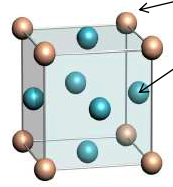
\includegraphics[width=0.1\textwidth]{FCC}                                                \\
HCP & $FE=0.74$ , $IC=12$ y $a=2R$ & 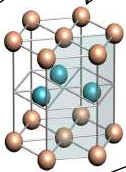
\includegraphics[width=0.1\textwidth]{HCP}                            
\end{tabular}
\end{table} \\
No obstante estas estructuras presentan huecos:
\begin{itemize}
	\item[BCC] \textbf{Octaedricos} las caras y mitad de la arista. 6/celda. $r=0.155$ \\
	\textbf{Tetraédricos} 4 en cada cara. 12/celda. $r=0.291R$
	\item[FCC] \textbf{Octaedricos} en el centro y mitad de la arista. 4/celda. $r=0.414R$ \\
	\textbf{Tetraédricos} en un cuarto de diagonal. 8/celda. $r=0.225R$
	\item[HCP] \textbf{Octaedricos} 3 en cada plano paralelo a la base. 6/prisma. $r=0.414R$ \\
	\textbf{Tetraédricos} en aristas e interior. 12/prisma. $r=0.225R$
\end{itemize}


	\subsection{Densidades de la estructura}
La densidad cristalina viene dada por la fórmula 
\[\rho = \frac{ZM}{N_AV}\]
La densidad reticular lineal dado una cierta dirección $[a,b,c]$ 
\[\rho_{[a,b,c]}=\frac{\text{Nº átomos en la dirección}}{\text{longitud de la línea}}\]
La densidad reticular planar dado un cierto plano $(a\ b\ c)$ 
\[\rho_{(a\ b\ c)}=\frac{\text{Nº átomos en el plano}}{\text{área del plano}}\]

	\subsection{Características}
	\begin{itemize}
		\item Sólidos a $T$ ambiente (-Hg)
		\item $EI$ baja
		\item $EN<2$
		\item Pocos $e^-$ en el último nivel
		\item $\rho$ altas
		\item Enlace fuerte
		\item Dúctiles y maleables
		\item Deformación elástica y plástica
		\item Brillo metálico y reflectividad
	\end{itemize}
	\subsection{Conductividad de calor y eléctrica}
	$R=$ Resistencia,  $\rho=$ Resistividad,  $\sigma=$ Conductividad,  $J=\frac{I}{A}$,  $n=e^-$ por unidad de volumen,  $\mu=$ movilidad de $e^-$ .
	\[\sigma=\frac{1}{\rho} \ \ \ \ R=\rho\frac{l}{A}\ \ \ \ J=E\sigma=nqv \implies \sigma=nq\mu\]
	Además $\rho$ varía en función de la temperatura de la siguiente manera:
	\[\rho=\rho_0(1+\alpha T)\]
	donde $\rho_0$ es la resisrividad a $T=0^0C$
	
	\subsection{Teoría de bandas}
	Es la aplicación de la Teoría de Orbitales Moleculares a los metales.\\ \\
	Los $e^-$ de la capa de valencia se comparten, y sus orbitales moleculares tienen energías tan próximas que se forma una banda.\\ \\
	Las bandas se dividen en:
	\begin{itemize}
		\item \textbf{Banda de valencia} formada por los orbitales atómicos de valencia.
		\item \textbf{Banda de conduccioón} formada por los orbitales atómicos vacíos.
	\end{itemize}
	Estas bandas poeden solaparse energéticamente.
	
		\subsubsection{Conductor}
		En los conductores la banda de valencia está semillena o llena, pero se encuentra solapada con la banda de conducción. \\
		Por esta razón los $e^-$ tienen espacio y se conduce la electricidad.
		\subsubsection{Aislante}
		En los aislantes existe una separación importante entre la banda de valencia y la de conducción.\\
		Por esta razón no conducen la electricidad.
		\subsubsection{Semiconductores}
		En los semiconductores la diferencia de energía entre las bandas $E_g\leq 1eV$.\\ \\
		Existen dos tipos de semiconductores:\\ \\
		Los \textbf{intrínsecos} estan formados por un solo átomo \\ \\
		Los \textbf{extrínsecos} se consiguen mediante un proceso de dopaje
		\begin{itemize}
			\item Tipo P: se emplean elementos con 3 $e^-$ de valrncia (B, In, Ga)
			\item Tipo N: se emplean elemontos con 5 $e^-$ de valencia (P, As, Sb)
		\end{itemize}
		
		
\section{Metales y aliaciones}
	\subsection{Aleaciones}
	Aleación $=$ Disolución sólida de dos o más elementos, uno de los cuales es un metal.\\
	\\
	Distinguimos los siguientes tipos:
	\begin{itemize}
		\item \textbf{Sustitutivos ($Ag, Au$)}\\
		El minoritaro se coloca en las posiciones del mayoritario.\\
		Para que tenga solubilidad total ha de cumplir las \textbf{Reglas de Hume-Rothery}
		\begin{itemize}
			\item[1)] Que todos los metales tengan la misma estructura cuando son puros.
			\item[2)] Variación de radios $< 15\%$.
			\item[3)] $EN$ similar y misma valencia.
		\end{itemize}
		\item \textbf{Intersticial (Acero $Fe,C$)}\\
		Átomos pequeños se situan en los huecos de la estructura cristalina de los grandes.
		\item \textbf{Intermetálicos ($TiAl$, $MgB_2$)} \\
		Formado por al menos un metal. Estructura diferente de los puros.		
	\end{itemize}
	
	\subsection{Diagramas de fase}
	\begin{figure}[h!]
\centering
\begin{subfigure}[b]{0.45\linewidth}
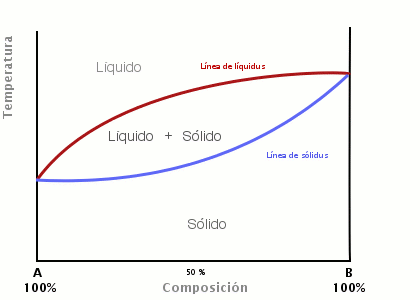
\includegraphics[width=\linewidth]{Diagrama_sol_total}
\caption{Solubilidad total $(Cu-Ni)$}
\label{fig:westminster_lateral}
\end{subfigure}
\begin{subfigure}[b]{0.45\linewidth}
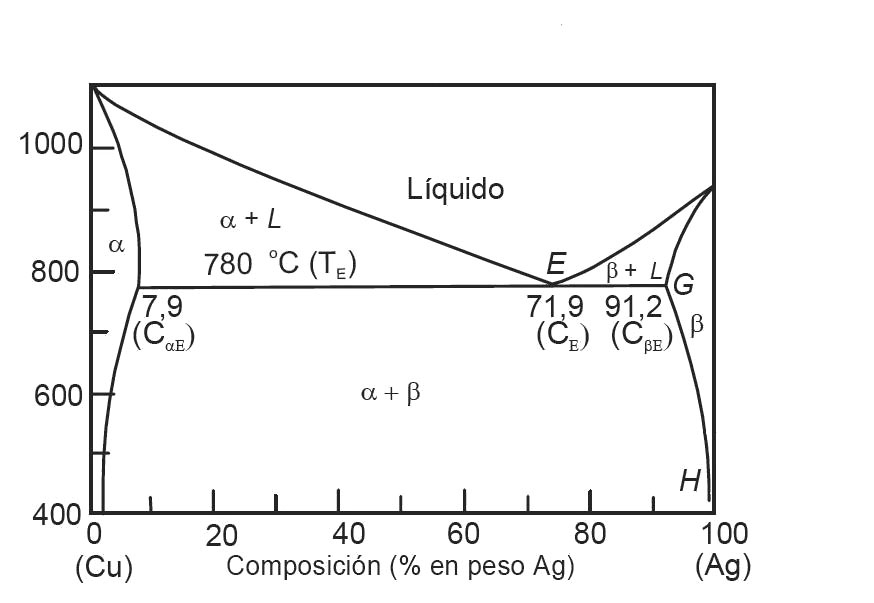
\includegraphics[width=\linewidth]{diagrama_sol_parcial}
\caption{Solubilidad parcial $(Cu-Ag)$}
\label{fig:westminster_aerea}
\end{subfigure}
\label{fig:westminster}
\end{figure}

\begin{figure}[h!]
\centering
\begin{subfigure}[b]{0.45\linewidth}
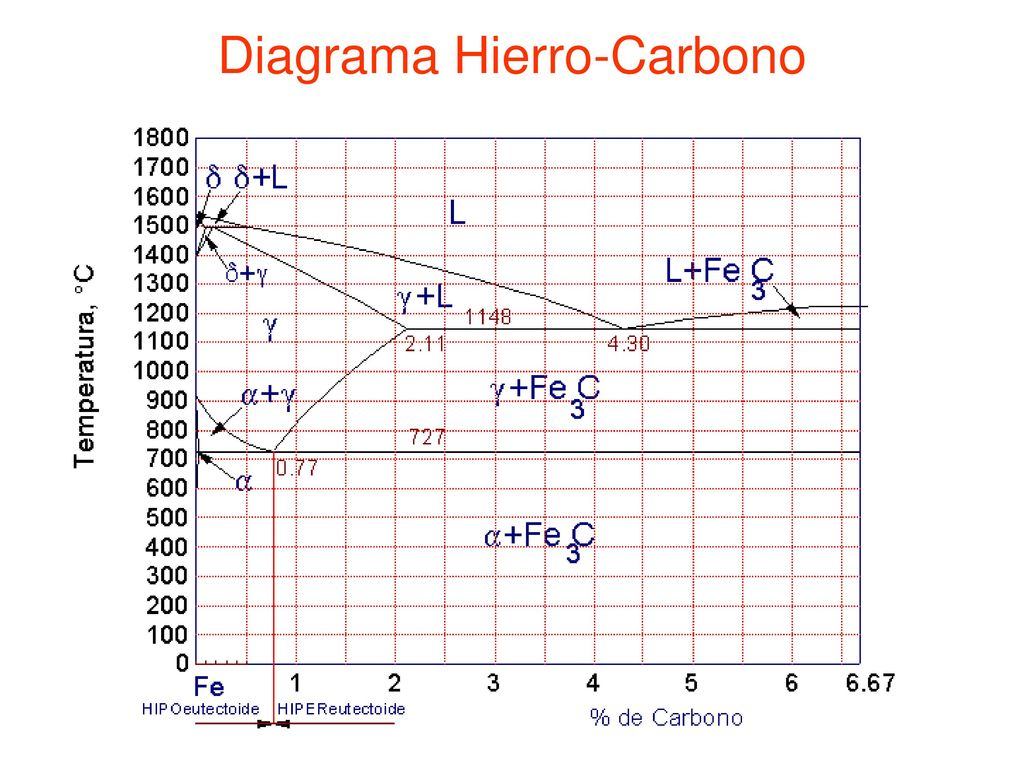
\includegraphics[width=\linewidth]{Diagrama_intersticial}
\caption{Compuesto intersticial $(Fe-C)$}
\label{fig:westminster_lateral}
\end{subfigure}
\begin{subfigure}[b]{0.45\linewidth}
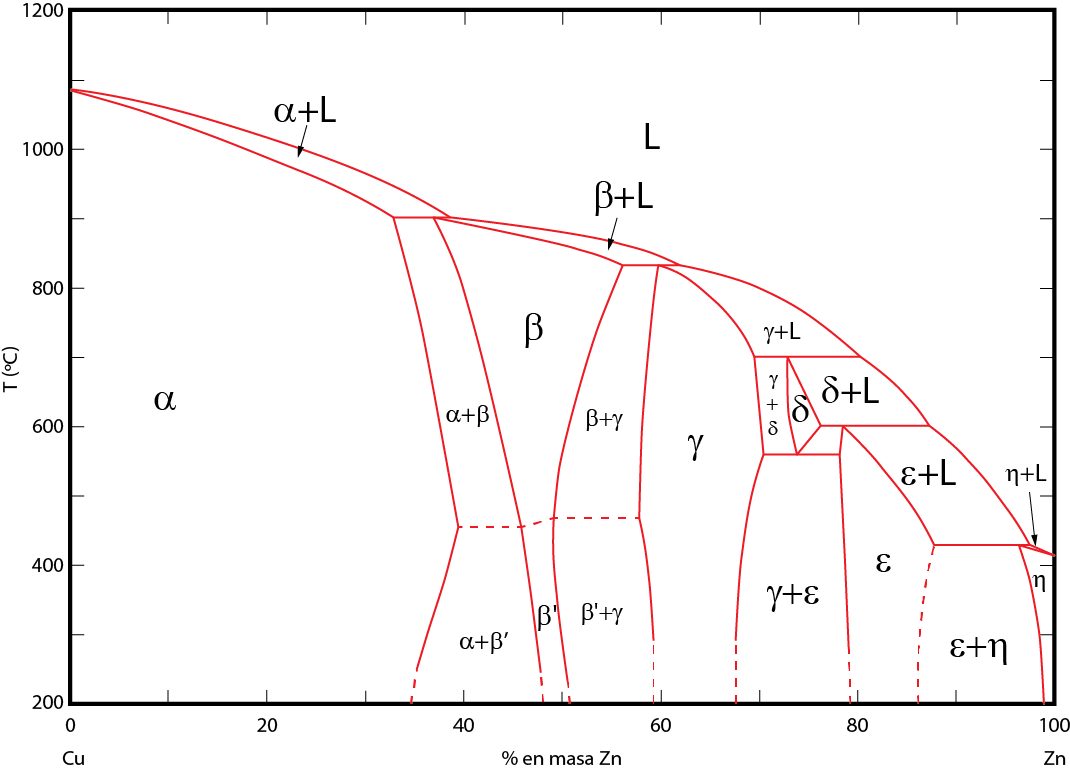
\includegraphics[width=\linewidth]{Diagrama_intermetalico}
\caption{Compuesto intermetálico $(Cu-Zn)$}
\label{fig:westminster_aerea}
\end{subfigure}
\label{fig:westminster}
\end{figure}

\section{Enlace iónico}	
	\subsection{Estructura de los compuestos iónicos}
	Tendremos un $IC$ diferente para el anión y el catión. $R_a>R_c$.
	\textbf{Reglas de Pauling}:
	\begin{itemize}
		\item La distacia catión anión $= R_a+R_c$
		\item Cada ión tiende a rodearse del mayor número de iones contrarios
	\end{itemize}
	$R_c/R_a$ indica el $IC$ (Mirar tabla de $IC$ en el formulario)
	
	\subsection{Estructuras modelo}
		\begin{itemize}
			\item[$\mathbf{AX}$]
			\begin{itemize}
				\item $\mathbf{IC=4 \ (ZnS)}$\\
				Estructura de los aniones FCC. Los cationes se colocan en 4 huecos (tetraédricos).\\
				Tangente en la diagonal $\sqrt{3}a=4R^-+4R^+$
				\item $\mathbf{IC=6 \ (NaCl)}$\\
				Estructura de los aniones FCC. Los cationes se colocan en los huecos (mitad de las aristas y centro).\\
				Tangente en la arista $a=2R^-+2R^+$
				\item $\mathbf{IC=8 \ (CsCl)}$\\
				Estructura de los aniones cúbica primitiva. El catión se coloca en el hueco del centro.\\
				Tangente en la diagonal $\sqrt{3}a=2R^-+2R^+$
			\end{itemize}
			
			\item[$\mathbf{A_mX_p}$]
			\begin{itemize}
				\item $\mathbf{IC=4 (cation) \ (Na_2O)}$ (Antifluorita)\\
				Estructura de los aniones FCC. Los cationes se colocan en los huecos (tetraédricos).\\
				Tangente en la diagonal $\sqrt{3}a=4R^-+4R^+$
				\item $\mathbf{IC=8 (cation) \ (CaF_2)}$ (Fluorita)\\
				Estructura de los cationes FCC. Los aniones se colocan en los huecos (tetraédricos).\\
				Tangente en la diagonal $\sqrt{3}a=4R^-+4R^+$
			\end{itemize}
			\item[$\mathbf{A_mB_nX_p}$]
			\begin{itemize}
				\item \textbf{Perovskita} $\mathbf{CaTiO_3}$ \\
				Estructura de $Ca$ cúbica primitiva. $O$ en las caras. $Ti$ en el centro. \\
				Estructura de $Ti$ cúbica primitiva. $O$ en las aristas. $Ca$ en el centro.
			\end{itemize}
		\end{itemize}
		
	\subsection{Ciclo de Born-Haber}
	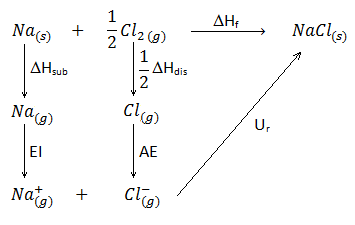
\includegraphics[scale=0.9]{Born_Haber}
	
	Otro método para conseguir la Enegía Reticular (esta vez de manera teórica) es a traves de la ecuación de la ecuación de \textbf{Born-Landé}
	\[U=-\frac{AN_Ae^2z_Az_C}{4\pi \varepsilon_0 d_{AC}}\left(1-\frac{1}{n}\right)\]
	\subsection{Propiedades del enlace iónico}
	\begin{itemize}
		\item Alto punto de fusión
		\item Duros y frágiles
		\item Aislantes, pero conductores en disolución con agua
		\item Solubles en agua ($\Delta H_{disolucion}=-U+\Delta H_{vaporizacion}+\Delta H_{solvatacion}$)
		\item Polarización. \textbf{Reglas de Fajans}
		\begin{itemize}
			\item[1)] + carga ó - radio $\implies$ catión + polarizado
			\item[2)] + carga ó + radio $\implies$ anión + polarizado
			\item[3)] Sin configuración de gas noble $\implies$ + polarización
		\end{itemize}
	\end{itemize}
	
\section{Cinética}
	\subsection{Velocidad de la reacción}
	\[aA \ + \ bB\ \to \ cC \ + \ dD\]
	\[r=-\frac{1}{a}\frac{d[A]}{dt}=\cdots=\frac{1}{d}\frac{d[D]}{dt} \ \ \ \ \ \ \ \ r=k[A]^\alpha[B]^\beta \ \ \ \ \ \ \ orden = \alpha + \beta\]
	El tiempo de vida media es el tiempo que tarda en reducirse a la mitad $t_{1/2}: \ \ [A]\to [A]/2$\\ 
	\\
	\subsection{Solución de la velocidad para distintos órdenes}
	\textbf{Orden 0}
	\[[A]=[A]_0-akt\]
	\\
	\textbf{Orden 1}
	\[ln[A]=ln[A]_0-akt\]
	\\
	\textbf{Orden 2} \\
	Si $a=b$ y $[A]_0=[B]_0$
	\[\frac{1}{[A]}=\frac{1}{[A]_0}+akt\]
	Si no se cumple alguna de las anteriores
	\[\frac{1}{a[B]_0-b[A]_0}ln\left(\frac{[A]_0[B]}{[B]_0[A]}\right)=kt\]
	
	\subsection{Factores que afectan a la velocidad}
	\begin{itemize}
		\item[1)] \textbf{Temperatura}.
		\[\text{Ecuación de Arrhenius   } k= Ae^{\frac{-E_a}{RT}}\]
		\item[2)] \textbf{Concentración de los reactivos}. Numero de colisiones.
		\item[3)] \textbf{Naturaleza de los reactivos}.
		\item[4)] \textbf{Grado de división}. En gas o líquido hay más colisiones. En sólido depende de la superfície de contacto.
		\item[5)] \textbf{Catalizadores}.
	\end{itemize}
	
	\subsection{Tipos de reacciones}
	\textbf{Reacciones elementales}\\
	Suceden en una sola etapa. La molecularidad es la suma de los coeficientes de los reactivos. \\
	\\
	\textbf{Reacciones complejas}
	Se llevan a cabo en diferentes etapas. Aparecen sustancias que no son reactivos ni productos llamadas intermedios de reacción. La velocidad depende de la etapa lenta.
	
\section{Acido Base}
	\subsection{Definiciones}
	\begin{itemize}
		\item \textbf{Arrhenius} \\
		Ácido = especie que cede $H^+$ cuando se disuelve en agua
		Base = especie que cede $OH^-$ cuando se disuelve en agua
		\item \textbf{Bronsted Lowry} \\
		Ácido = especie que es capaz de ceder $H^+$ cuando se disuelve en in disolvente
		Base = especie que es capaz de ceder $OH^-$ cuando se disuelve en un disolvente
		\item \textbf{Lewis}\\
		Ácido = compuesto capaz de recibir $e^-$
		Base = compuesto capaz de ceder $e^-$ 
	\end{itemize} 
	
	En cada reacción hay un elemento y su ácido/base conjugada
	\begin{itemize}
		\item $HCN$ es el ácido conjugado de $CN^-$
		\item $CN^-$ es la base conjugada de $HCN$
	\end{itemize}
	La constante de acidez $K_a$ y el $pH$ en la reacción $HCN \ \ \to \ \ CN^-\ \ + \ \ H^+$
	\[K_a=\frac{[CN^-][H^+]}{[HCN]} \ \ \ \ \ \ K_w=[H^+][OH^-]=10^{-14} \ \ \ \ pH=-log[H^+]\]
	
	\subsection{Planteamiento de un ejercicio}
	\textbf{Paso 1}\\
	Escribir todas las reacciones involucradas (incluida la hidrólisis del agua)\\
	\\
	\textbf{Paso 2}\\
	Escribir los equilibrios ($K_a$ y $K_w$) y las los balances de masa y carga (bm, bc)\\
	\\
	\textbf{Paso 3}\\
	Resolver el sistema o usar el diagrama logarítmico
	\begin{itemize}
		\item 2 reacciones: ácido/base fuerte ($HX$ o $XOH$) y agua $\Rightarrow$ resolver sistema
		\item 2 reacciones: ácido/base débil y agua $\Rightarrow$ gráfica logarítmica, despreciar $[OH^-]/[H^+]$ y resolver sistema
		\item Más de 2 reacciones: sares se disocian completamente (si no nos dan $K_s$). Despreciar $[OH^-]$ y $[H^+]$ en bc. Resolver sistema y razonar con diagrama logarítmico.
	\end{itemize}
	
	\subsection{Neutralización}
	Ácido + Base $\longrightarrow$ Sal + $H_2O$ \\
	Se utiliza para encontrar el punto de equivalencia en en una disolución.		
	
	\subsection{Disoluciones tampón}
	Formados por ácido debil y su base conjugada $\Rightarrow$ $pH$ constante al adicionar ácido/base.\\
	\\
	Para el cálculo debemos realizar el equilibrio de nuevo. Normalmente nos darán una sal (se disocia completamente), y debemos añadir en equilibrio su correspondiente ácido/base, que se disociará con la $K_a/K_b$	
	\section{Reacciones Redox}
	Lo primero que hay que hacer es ajustar las semirreacciones de oxidación (aumenta la valencia) y reducción (disminuye la valencia).
	
	\subsection{Ecuación de Nernst}
	Tenemos una reacción donde la \textbf{r}educción se realiza en el \textbf{c}átodo y la \textbf{o}xidación en el \textbf{á}nodo. La reacción se dará si
	\[\varepsilon=E_{catodo}-E_{anodo}>0\]
	\\
	\textbf{Ecuación de Nernst}. Se utiliza cuando la concenntración molar es diferente de $1M$\\
	\[\varepsilon=\varepsilon^0 - \frac{0.059}{n}logQ\]
	
	\subsection{Tipos de reacciones redox}
	\subsubsection{Celda galvánica}
	\[Anodo \ \ \ \ Fe \longrightarrow Fe^{2+} + 2e^- \ \ \ \ \ E^0 = -0,44V\]
	\[Catodo \ \ \ \ Cu^{2+} + 2e^- \longrightarrow Cu \ \ \ \ \ E^0 = 0,34V \]
	
	\subsubsection{Celda de concentración}
	\[Anodo \ \ \ \ Cu \longrightarrow Cu^{2+}(0.1M) + 2e^- \]
	\[Catodo \ \ \ \ Cu^{2+}(1M) + 2e^- \longrightarrow Cu \]
	Aplicando la ecuación de Nernst ($\varepsilon^0= 0$ porque la especie que se reduce es la misma que se oxida)
	\[\varepsilon = -\frac{0.059}{2}logQ=-\frac{0.059}{2}log\frac{0.1}{1}=0.029V\]
	
	\subsubsection{Celda de aireo diferencial}
		\[Anodo \ \ \ \ 2H_2O \longrightarrow O_2(0.1atm) + 4H^+ + 4e^- \]
	\[Catodo \ \ \ \ O_2(1atm) + 4H^+ + 4e^- \longrightarrow 2H_2O \]	
	Aplicando la ecuación de Nernst ($\varepsilon^0= 0$ porque la especie que se reduce es la misma que se oxida)
	\[\varepsilon = -\frac{0.059}{4}logQ=-\frac{0.059}{4}log\frac{0.1 \cdot [H^+]^4}{1\cdot [H^+]^4}=0.015V\]
	
	
	\subsubsection{Determinación del pH}
	Se basa en el hecho de que la reacción:
	\[H^+ \longrightarrow H  \ \ \ \ \ \varepsilon=-\frac{0.059}{1}log\frac{1}{[H^+]}=-0.059pH\]
	tiene un potencial que podemos medir y calcular así el pH.
	
	\subsection{Diagramas}
	\subsubsection{Digramas de Latimer}	
	Indican el potencial estandar de reducción cuando el elemento se reduce:
	\[ClO_4^- \xrightarrow[+1.20V]{}  ClO_3^- \xrightarrow[+1.18V]{} + HClO_2 \xrightarrow[+1.65V]{} HClO \xrightarrow[+1.67V]{}  Cl_2 \xrightarrow[+1.36V]{} Cl^-\]
	Para calcular el potencial estándar se utiliza
	\[E^{\circ}_{+7\to +3} = \frac{n_{+7 \to +5}E^{\circ}_{+7 \to +5} + n_{+5 \to +3}E^{\circ}_{+5 \to +3}}{n_{+7 \to +5} + n_{+5 \to +3}} = \frac{2\times 1.20+ 2\times 1.18}{2+2} = 1.19V\]
	\\	
	\subsubsection{Digramas de Frost}
	\begin{wrapfigure}{r}{0.30\textwidth}
    	\centering
    	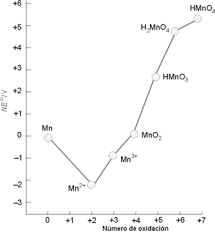
\includegraphics[width=0.20\textwidth]{Frost}
	\end{wrapfigure}
Se representa el Potencial estándar multiplicado por el número de oxidación en función del estado de oxidación. \\ \\
Hay \textbf{desproporción} si una especie está por encima de la recta que une a sus vecinas \\ 
Hay \textbf{comproporción} si una especie está por debajo de la recta que une a sus vecinas \\ 
La más \textbf{estable} es la más baja de todas en el diagrama
\\
	\subsubsection{Digramas de Pourbaix}
	En un diagrama de pourbaix tenemos 3 tipos de rectas que separan las zonas:\\
	\textbf{Horizontales} \\
	Cambios eléctricos. Debemos plantear la ecuación de Nernst y ver cual es el potencial al que se da la corrosión ($[M^+]=10^{-6}M$). \\
	\\
	\textbf{Verticales}\\
	Cambios ácido-base. Debemos realizar el equilibrio y encontrar el pH en el que se da la reacción.\\
	\\
	\textbf{Transversales}\\
	Cambios electroquímicos. Planteamos la ecuación de Nerns y ponemos el potencial en función del pH.\\
	\\
	Tenemos también otras dos rectas discontinuas:\\
	\textbf{Agua desaireada}
	\[2H^+ + 2e^- \longrightarrow H_2 \ \ \ \Rightarrow \ \ \ E=-0.059pH\]	
	\textbf{Agua aireada}
	\[4H^+ O_2 + 4e^- \longrightarrow 2H_2O \ \ \ \Rightarrow \ \ \ E=E^0(O_2/H_2O)-0.059pH = 1.23-0.059pH\]	
	
	
\section{Importante para el examen}
Esta es una recopilación de cosas que le gusta poner a Iñaki en el examen y que ha dicho de pasada en clase. Son conceptos recurrentes que han salido en examenes anteriores.
	\subsection{Peste del Estaño}
	El $Sn$ tiene dos formas alotrópicas:
	\begin{itemize}
		\item \textbf{Estaño blanco ($\beta$)}. Estructura tetragonal y se encuentra a temperatura ambiente.
		\item \textbf{Estaño gris ($\alpha$)}. Estructura cúbica y se encuentra a $-30^0C$.
	\end{itemize}
	Cuenta la leyenda que esta fue una de las causas de la derrota de las tropas napoleónicas en la guerra contra la Rusia Zarista de 1812. Debido a las bajas temperaturas, los soldados vestian botones de estaño que sufrieron esta transformación y se desintegraron, imposibilitándoles  abrocharse la ropa.
	
	\subsection{Molécula de $NH_3$ y efecto túnel}
	\begin{wrapfigure}{r}{0.30\textwidth}
    	\centering
    	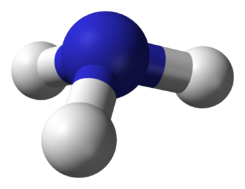
\includegraphics[width=0.20\textwidth]{nh3}
	\end{wrapfigure}
	Dada la geometría de la molécula de $NH_3$, tenemos un par no enlazante del $N$, por lo que la geometría es trigonal plana. \\
	Debido al efécto túnel este par puede pasar a través de la molécula e invertir la geometría (el par pasa a estar de arriba a abajo). \\
	
	\subsection{Momento dipolar de $NH_3$ y $NF_3$}
	Realizamos las estructuras de Lewis de las moléculas (ambas son trigonal plana). A priori nos podría parecer que al ser similares, $\mu(NH_3)<\mu(NF_3)$, ya que el $F$ es más electronegativo que el $H$. No obstante, en la molécula de $NF_3$, el vector del momento dipolar del par no elnazante y los del enlace $NF$ se anulan parcialmente dado que $F$ es más elecronegativo que $N$.\\
	Por todo esto tenemos que $\mu(NH_3)>\mu(NF_3)$. \\
	\\
	Nota: esto también sucede con otras moléculas como $H_2O$ y $OF_2$.
	
	\subsection{Función de probabilidad radial}
	Si nos dan una función de onda $\Psi$ en coordenadas polares podemos separarla en términos radiales y angulares:
	\[\Psi = re^{-\frac{r}{2a_0}}sin\theta cos\phi \Rightarrow \begin{cases} R(r)=re^{-\frac{r}{2a_0}} \\ Y(\theta, \phi) = sin\theta cos\phi \end{cases}\]
	Ahora definimos la función de densidad de probabilidad radial como
	\[P(r) = r^2R(r)^2\]
	Buscamos el máximo de la función $P(r)$, y en ese punto tendremos la probabilidad máxima de encontrar al electrón.
	
	\subsection{Promoción electrónica}
	Cuando se realiza la configuración electrónica tenemos dos excepciones donde se produce la promoción electrónica:\\
	\\
	$Cr: \ 1s^2 2s^2 2p^6 3s^2 3p^6 3d^5 4s^1$\\
	Vemos como en lugar de llenar el orbital $4s$, el último electrón se coloca semiocupando la $3d$.\\
	\\
	$Cu: \ 1s^2 2s^2 2p^6 3s^2 3p^6 3d^{10} 4s^1$\\
	Vemos como en lugar de llenar el orbital $4s$, el último electrón se coloca llenando la $3d$.
		
	
	
	
	


\end{document}






















